\documentclass[tikz]{memoir}

\usepackage{tikz}

\usepackage[EULERGREEK]{sansmath}

\makeatletter
\def\mute{x}
\def\open{o}
\newcounter{fretcounter}

\newcommand{\akkoord}[2]{
  \begin{tikzpicture}[font=\sffamily\sansmath]
  % Draw snares and frets (6 and 4)
  \draw[help lines] (0,0) grid (5,4);
  % \filldraw [fill=black] (1,1.5) circle [radius=0.5];
  % \draw [color=white] (1,1.5) node {\Large 1};
  % \draw (-1,3.5) node {\Large III};
  % \draw (0,2) to[out=20, in=160] (5,2);
  % \draw (3,4.5) node {\Large X};
  % \draw (2,4.5) node {\Large O};
  % \draw (0,-0.5) node {\Large $\flat$7};
  % Write name of chord
  \draw (2.5,5.5) node {\Huge #2};

  \setcounter{fretcounter}{0}
  \@tfor\fret:=#1\do
    {\ifx\fret\mute
      {\draw (\thefretcounter, 4.5) node {\Large X};}
    \else
      {\ifx\fret\open
        {\draw (\thefretcounter, 4.5) node {\Large O};}
      \else
        {\filldraw [fill=white] (\thefretcounter, 4.5-\fret) circle [radius=0.5];
        \draw (\thefretcounter, 4.5-\fret) node {\Large 1};}
      \fi}
    \fi
    \stepcounter{fretcounter}
    }
  \end{tikzpicture}
}
\makeatother

\begin{document}


\akkoord{3x3x3o}{G\textsubscript{$\triangle$}}


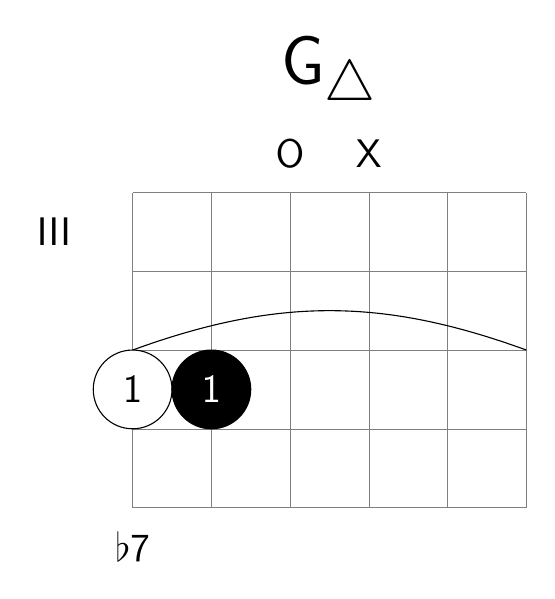
\begin{tikzpicture}[font=\sffamily\sansmath]
\draw[help lines] (0,0) grid (5,4);
\filldraw [fill=white] (0,1.5) circle [radius=0.5];
\draw (0,1.5) node {\Large 1};
\filldraw [fill=black] (1,1.5) circle [radius=0.5];
\draw [color=white] (1,1.5) node {\Large 1};
\draw (-1,3.5) node {\Large III};
\draw (0,2) to[out=20, in=160] (5,2);
\draw (3,4.5) node {\Large X};
\draw (2,4.5) node {\Large O};
\draw (0,-0.5) node {\Large $\flat$7};
\draw (2.5,5.5) node {\Huge G\textsubscript{$\triangle$}};
%\draw[step=0.5, gray, very thin] (-1.4,-1.4) grid (1.4,1.4);
%\draw (0,0) parabola (1,1.5) parabola[bend at end] (2,0);
%\draw (0,0) sin (1,1) cos (2,0) sin (3,-1) cos (4,0) sin (5,1);
\end{tikzpicture}
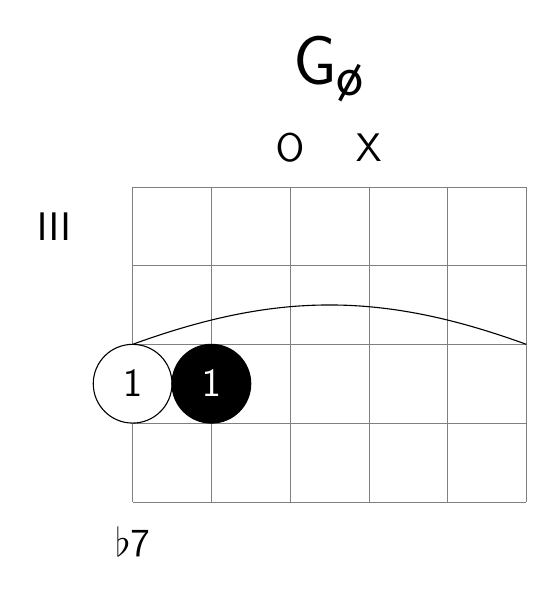
\begin{tikzpicture}[font=\sffamily\sansmath]
\draw[help lines] (0,0) grid (5,4);
\filldraw [fill=white] (0,1.5) circle [radius=0.5];
\draw (0,1.5) node {\Large 1};
\filldraw [fill=black] (1,1.5) circle [radius=0.5];
\draw [color=white] (1,1.5) node {\Large 1};
\draw (-1,3.5) node {\Large III};
\draw (0,2) to[out=20, in=160] (5,2);
\draw (3,4.5) node {\Large X};
\draw (2,4.5) node {\Large O};
\draw (0,-0.5) node {\Large $\flat$7};
\draw (2.5,5.5) node {\Huge G\textsubscript{\o}};
%\draw[step=0.5, gray, very thin] (-1.4,-1.4) grid (1.4,1.4);
%\draw (0,0) parabola (1,1.5) parabola[bend at end] (2,0);
%\draw (0,0) sin (1,1) cos (2,0) sin (3,-1) cos (4,0) sin (5,1);
\end{tikzpicture}
\end{document}
